\begin{frame}
\frametitle{Problem Statement-Circle Exercise}
\begin{enumerate}[label=(\roman*)]
\item In any $\triangle$ABC, if the angle bisector of $\angle$A and
perpendicular bisector of BC intersect, prove that they intersect on the circumcircle of the $\triangle$ABC

\textbf{Soln:}\\
  
\end{enumerate}
\begin{figure}
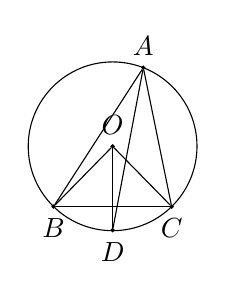
\begin{tikzpicture}[scale =0.3,>=stealth,point/.style = {draw, circle, fill = black, inner sep = 0.4pt},]
\draw (2.5,2.55155182)circle (3.57217254156cm);
\node (A) at (3.8,5.87877538)[point,label=above :$A$] {};
\node (B) at (0,0)[point,label=below :$B$] {};
\node (C) at (5,0)[point,label=below :$C$] {};
\node (D) at (2.5,-1)[point,label=below :$D$] {};
\node (O) at (2.5,2.55155182)[point,label=above :$O$]{};
\draw (A)--(B);
\draw (A)--(C);
\draw (A)--(D);
\draw (B)--(C);
\draw (B)--(O);
\draw (O)--(C);
\draw (O)--(D);
\end{tikzpicture}
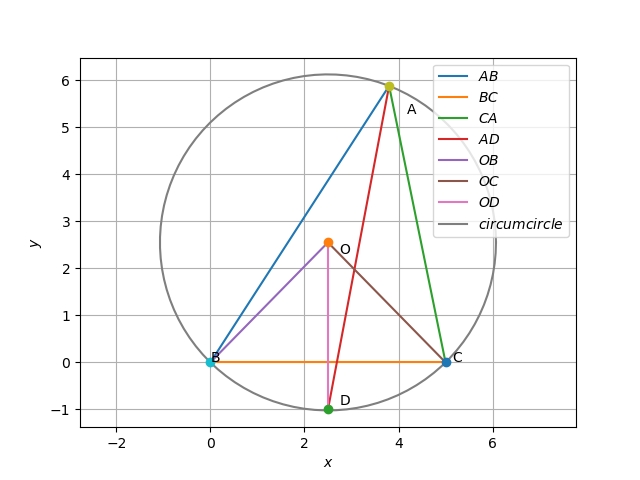
\includegraphics[scale=0.2]{./figs/cirexe.png}
\end{figure}
\end{frame}
\begin{frame}
\begin{align*}
\angle{BOC}= 2\angle{BAC}=2\angle{A} ...(1)\\
OB=OC\\
\angle{OEB}=\angle{OEC}\\
\triangle{BOE} \cong \triangle{COE}  ...(2)\\
\angle{BOE}+\angle{COE}=\angle{BOC}\\
\end{align*}
therefore,
\begin{align}
\angle{BOE}+\angle{BOE}=2\angle{A}\\
\angle{BOD}=\angle{BOE}=\angle{A}\\
\angle{BAD}=\frac{\angle{A}}{2}\\
2\angle{BAD}=\angle{A}\\
\angle{BOD}=2\angle{BAD}\\
\end{align}
\end{frame}